\documentclass{article}
\usepackage[utf8]{inputenc}
\usepackage{amsmath}
\usepackage{float}
\usepackage{graphicx}

\title{Project Milestone}
\author{Shenglan Qiao, Daniel L\'{e}vy}
\date{November 2015}

\begin{document}

\maketitle

\section{Introduction}
Automatic language classification is far from being a solved problem. Although simple methods can achieve almost perfect accuracy of classification under certain circumstances (McNamee 2005), discriminating between similar languages is still considered non-trivial. For example, Franco-Salvador et al. (2015) demonstrated that it is far from simple to classify blog posts from five different countries: Argentina, Chile, Mexico, Peru, and Spain. Classifying texts in Serbo-Croatian languages has also been particularly difficult. The difficulty of classification in this domain of language detection justifies searches for better methods.

We aim to implement and improve a state-of-art method for classifying similar languages and regional varieties. Specifically, we are attempting the Discriminating between Similar Language (DSL) Shared Task 2015. This challenge is to build a system that can discriminate sentences in 13 different languages from 6 language groups.

The task provides a data set for training the system and evaluating its performance. The training set contains 250,000 labeled sentences extracted from journalistic corpora. The data set also includes a development set and a variety of labeled and unlabeled test sets. The following language groups are included.

\begin{itemize}
\item South-Eastern Slavic (se\_s): Bulgarian (bg), Macedonian (mk)
\item South-Western Slavic (sw\_s): Bosnian (bs), Croatian (hr), Serbian (sr)
\item West Slavic (w\_s): Czech (cz), Slovak (sk)
\item Spanish(es): Argentine Spanish (esar), Peninsular Spanish (eses)
\item Portuguese (pt): Brazilian Portuguese (ptbr), European Portuguese (ptpt)
\item Austronesian (aus): Indonesian (id), Malay (my)
\end{itemize}

To emulate a realistic language identification setup additional texts from various other languages are added to the data set. They are labelled with the language code 'xx'. A robust language identification system should be able to identify a test example as an 'unknown language' it has not seen before.

\section{A Simple Method}
In order to understand the challenges of language identification, we first implemented a word frequency method. From the training set, it found the 1000 most common words for each language and computed for each word the frequency of its occurrence in the training corpus. Thus from the training set we obtained 13 1000-dimensional vectors, $x_{n}$ for language $n$. To predict the language of a test example, we represented it first as $x'_{n}$, a 1000-dimensional vector for language $n$. The ith component of $x'_n$ was one if the $i$th most common word from language $n$ was present in the test example and was zero otherwise. For each language $n$ we computed a score equal to the dot product of $x_n$ adn $x'_n$. The language with the highest score is then determined as the label for the test example. For simplicity, we excluded the 'xx' category in the training set. McNamee shown in 2005 that it is effective for languages that are largely distinct.

This method was computational efficient and obtained virtually perfect results for differentiating among five out of the six language groups (figure~\ref{fig:simple1}). It did not do as well on the West Slavic group. However, within language groups this method did not fare well (figure~\ref{fig:simple2}). For certain groups, it tended to identify examples as a 'default' language within the group thus driving down the identification accuracy of other languages within that same group. For instance, within the Spanish group, examples were much more likely to be labeled as Peninsular Spanish despite that there were equal number of test examples in both varieties of the language.

Results from this naive method are elucidating. They suggest that one-grams consisting of single words do not sufficiently capture the subtle syntactic differences between similar languages. We need to include longer word n-grams or character n-grams as features. In order to balance the need for more features and our limited computation resources, we decide to adopt an ensemble of classifiers, each having a different set of features and can be trained in parallel. We will combine the decisions from ensemble when predicting the label of a training example.

\begin{figure}[h!]\label{fig:simple1}
  \centering
    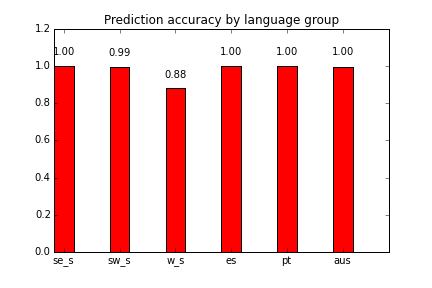
\includegraphics[width=0.7\textwidth]{acc_lg_group.png}
    \caption{Accuracy of the naive method in differentiating trest example from different language groups}
\end{figure}


\begin{figure}[h!]\label{fig:simple2}
  \centering
    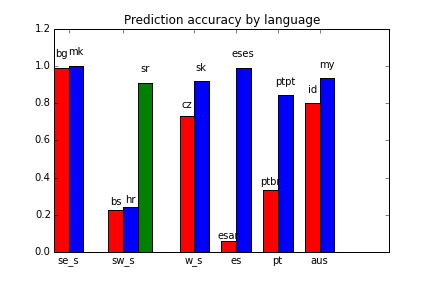
\includegraphics[width=0.7\textwidth]{acc_lg.png}
    \caption{Differentiating within the language groups are more difficult. The simple method does poorly because it tends to identify a 'default' language for certain groups.}
\end{figure}


\section{A More Advanced Method}
talk about the multi-classifier method

\section{Progress and Challenges}
What we find challenging for now and how we are going to fix them

\end{document}
